\documentclass[sigconf]{acmart}

\usepackage{graphicx}
\usepackage{pgfplots}

\usepackage{amssymb}
\usepackage{amsmath}
\usepackage{booktabs}

\usepackage{enumitem}
\usepackage{marginnote}
\setlength{\marginparwidth}{15mm}
\setlength{\marginparsep}{1mm}
\definecolor{darkblue}{rgb}{0.0,0.0,0.3}
\newcommand\todo[1]{\textcolor{blue}{[TODO: #1]}}
\newcommand\TODO[1]{\textcolor{blue}{\small [#1]}}
\newcommand\TODOM[1]{\marginpar{\color{blue}\renewcommand{\baselinestretch}{0.8}\tiny\tolerance=100000\hyphenpenalty=0\raggedright #1}}

% Input Graph

\def\iG{G}  % Input graph
\def\iV{V}  % Input nodes
\def\iv{v}  % Input node
\def\iE{E}  % Input edges
\def\ie{e}  % Input edge

% Drawing

\newcommand\drawing[1]{\mathcal{D}_{#1}}  % Drawing of graph
\newcommand\initdrawing[1]{\drawing{#1}^*}  % Drawing of graph

\def\drawingcurvesym{c}  % edge curve part of drawing
\def\drawingpossym{p}    % node position part of drawing

\newcommand\drawingcurve[1]{\drawingcurvesym(#1)}  % Drawing curve of argument edge
\newcommand\drawingpos[1]{\drawingpossym(#1)}  % Drawing pos urve of argument node

% Grid

\def\gScale{C}
\def\gmind{\hat d}


% Octilinear grid graph

\def\gG{\Gamma}  % Grid graph
\def\gV{\Psi}  % Grid graph nodes
\def\gv{\psi}  % Grid graph node
\def\gE{\Omega}  % v edges
\def\ge{\omega}  % Grid graph edge

\newcommand\ggv[2]{\gv_{#1, #2}}  % Grid node at #1, #2
\newcommand\gpv[3]{\gv_{#1, #2}^{#3}}  % Port #3 node at #1, #2
\newcommand\gse[3]{\ge_{#1, #2}^{#3}}  % Sink edge #3 node at #1, #2
\newcommand\gbe[4]{\ge_{#1, #2}^{#3, #4}}  % Bend edge for angle #4 at port #3 at node at #1, #2

\def\gPath{p}    % path on grid graph
\def\gPathOcti{p'}    % path on octilinear grid graph

\newcommand\gPturn[1]{c_{#1}}  % Turn penalty
\newcommand\gPturnEdge[1]{c'_{#1}}  % Turn penalty
\def\gHopcost{c_h}    % Hop cost in grid graph
\def\gHopcostOcti{c'_h}    % Hop cost in grid graph
\def\gSinkcost{c_s}    % Hop cost in grid graph
\newcommand\gPcost[1]{c(#1)}  % Path cost
\newcommand\gPcostOcti[1]{c'(#1)}  % Octilinear path cost

% ILP

\newcommand\gvused[2]{x_{#1#2}}	% bin. decision variable whether grid node #1 is assigned to input node #2
\newcommand\geused[2]{x_{#1#2}}	% bin. decision variable whether grid edge #1 is used be input edge #2

\newcommand\dir[2]{\delta_{#1#2}}	% variable telling the direction of edge #2 at node #1
\newcommand\dirdiff[2]{\Delta_{#1#2}}	% variable telling the direction difference of edge #1 and edge #2

\newcommand\bend[3]{\Delta_{#1#2}^{#3}}	% variable telling the direction difference of edge #1 and edge #2

\def\ldeg{\text{ldeg}}

\usepackage{tikz}
\usetikzlibrary{calc,trees,positioning,arrows,chains,shapes.geometric,%
  decorations.pathreplacing,decorations.pathmorphing,shapes,%
  matrix,shapes.symbols,plotmarks,decorations.markings,shadows}

\DeclareMathOperator{\atantwo}{atan2}

% Copyright
%\setcopyright{none}
%\setcopyright{acmcopyright}
%\setcopyright{acmlicensed}
\setcopyright{rightsretained}
%\setcopyright{usgov}
%\setcopyright{usgovmixed}
%\setcopyright{cagov}
%\setcopyright{cagovmixed}

% DOI
%\acmDOI{10.475/123_4}

% ISBN
%\acmISBN{123-4567-24-567/08/06}

%Conference
\acmConference[SIGSPATIAL '20]{SIGSPATIAL '20}{November 3-6 2020}{Seattle, Washington, USA}
\acmYear{2018}
\copyrightyear{2018}

\renewcommand{\topfraction}{0.96}
\renewcommand{\textfraction}{0.01}
\renewcommand{\floatpagefraction}{0.96}

\def\Hms{\makebox[1.6mm][l]{\hspace{0.2mm}\footnotesize ms}}
\def\Hs{\makebox[1.6mm][l]{\hspace{0.2mm}\footnotesize s}}
\def\Hk{\makebox[1.6mm][l]{\hspace{0.2mm}\footnotesize k}}
\def\Hm{\makebox[1.6mm][l]{\hspace{0.2mm}\footnotesize m}}
\def\Hh{\makebox[1.6mm][l]{\hspace{0.2mm}\footnotesize h}}
\def\Hhline{\\[.7mm]\hline}

\makeatletter
\DeclareRobustCommand*\cal{\@fontswitch\relax\mathcal}
\makeatother

\DeclareMathOperator*{\argmin}{\arg\!\min}
\DeclareMathOperator*{\argmax}{\arg\!\max}
\DeclareMathOperator*{\TED}{TED}
\DeclareMathOperator*{\lev}{lev}

\begin{document}
\title{Some Title}

\author{Hannah Bast}
\affiliation{%
  \institution{University of Freiburg}
  \city{Freiburg}
  \state{Germany}
}
\email{bast@cs.uni-freiburg.de}

\author{Patrick Brosi}
\affiliation{%
  \institution{University of Freiburg}
  \city{Freiburg}
  \state{Germany}
}
\email{brosi@cs.uni-freiburg.de}

\author{Sabine Storandt}
\affiliation{%
  \institution{University of Konstanz}
  \city{Konstanz}
  \state{Germany}
}
\email{sabine.storandt@uni-konstanz.de}

\begin{abstract}
We investigate the problem of finding the most likely geographic path a public transit vehicle (road-, rail- or water-bound) will take between a sorted list of given station coordinates. This sparse map-matching task frequently arises when real-world schedule data (where the geographic information often only consists of imprecise station locations) should be prepared for visualization, for example in route-planners or in transit-map drawing. It can also be a valuable pre-processing step for the closely related problem of on-line matching live passenger GPS data (e.g. from a smartphone) to a specific public transit vehicle. Our approach is implemented in a publicly-available tool called \emph{pfaedle} which matches arbitrary transit schedules (given as GTFS files) against geographic data from OpenStreetMap with high precision. We test our approach by comparing vehicle paths published by the transit agencies of several cities against the paths found by our tool. Previous work either primarily considered non-sparse private transport scenarios, did not handle inter-hop turn-restrictions, did not find a globally optimal path and/or lacked an extensive evaluation against real-world schedule data.
\end{abstract}

%
% The code below should be generated by the tool at
% http://dl.acm.org/ccs.cfm
% Please copy and paste the code instead of the example below.
%
\begin{CCSXML}
<ccs2012>
<concept>
<concept_id>10002951.10003227.10003236.10003237</concept_id>
<concept_desc>Information systems~Geographic information systems</concept_desc>
<concept_significance>500</concept_significance>
</concept>
<concept>
<concept_id>10003752.10003809.10003636.10003811</concept_id>
<concept_desc>Theory of computation~Routing and network design problems</concept_desc>
<concept_significance>500</concept_significance>
</concept>
</ccs2012>
\end{CCSXML}

\ccsdesc[500]{Information systems~Geographic information systems}
\ccsdesc[500]{Theory of computation~Routing and network design problems}

\keywords{Public Transit, Map Matching, Schedule Data, GTFS}

\maketitle

\section{Introduction}

Maps of public transit networks usually depict the lines in a schematized way to ensure readability.
In 1931, Harry Beck presented his idea to draw the London subway lines as alternating sequences of horizontal, vertical and diagonal line segments \cite{garl94}.
This octilinear design has since become the de facto standard and its usage goes beyond the cartographic representation of public transit networks.

The high practical relevance of these maps has lead to numerous approaches to render them automatically.
We give an overview of existing work in Section~\ref{SEC:related}.
However, existing methods usually do not guarantee octilinear results, require impractically long solution times and/or only allow a small fixed number of bends (or none at all) along edges in the final drawing.
This leads to several restrictions in their practical applicability.
In particular, previous work which guaranteed octilinear results often did not have solution times fast enough to be used interactively in a map editor.
Additionally, we are not aware of any previous work which allows octilinear drawings to approximate the real geographical courses of a line between stations, which is a requirement if the final maps should be combined with either existing maps or satellite imagery.
In this work, our goal is to overcome these restrictions.

\begin{figure}
    \centering
	\vspace{-0.6cm}
	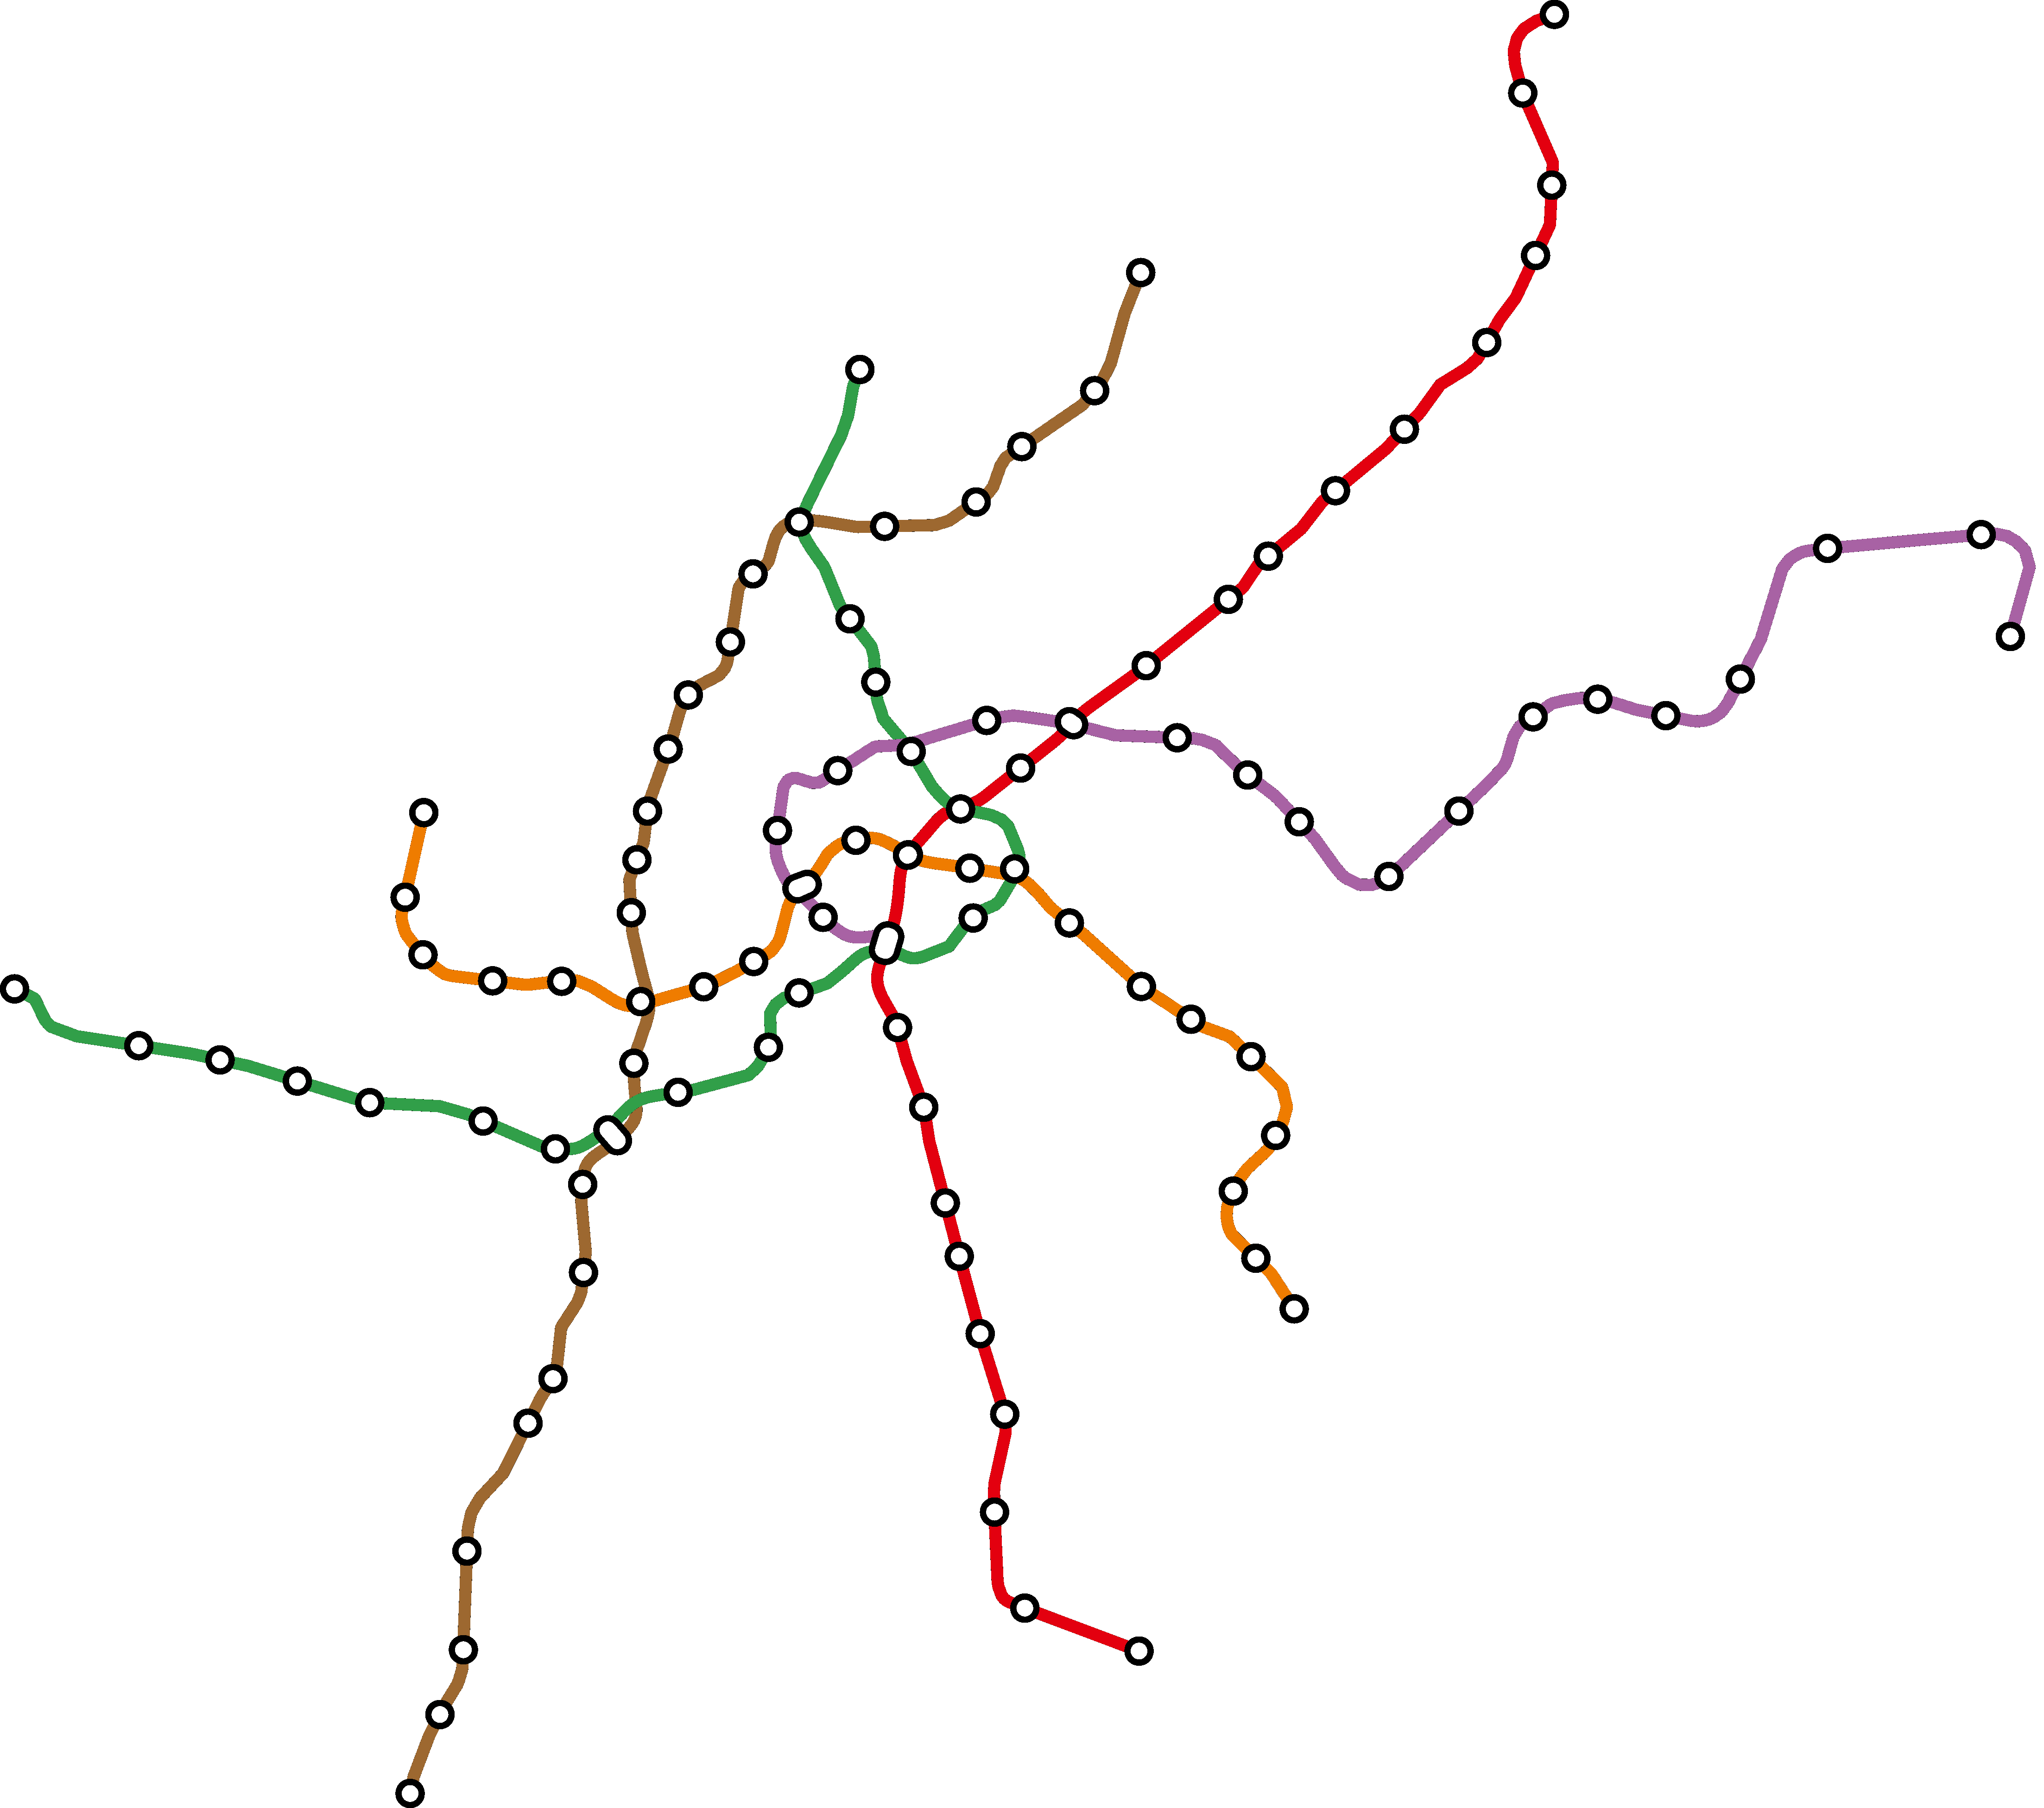
\includegraphics[width=0.27\textwidth]{figures/octi_input.pdf}
	\hspace{-1.3cm}
	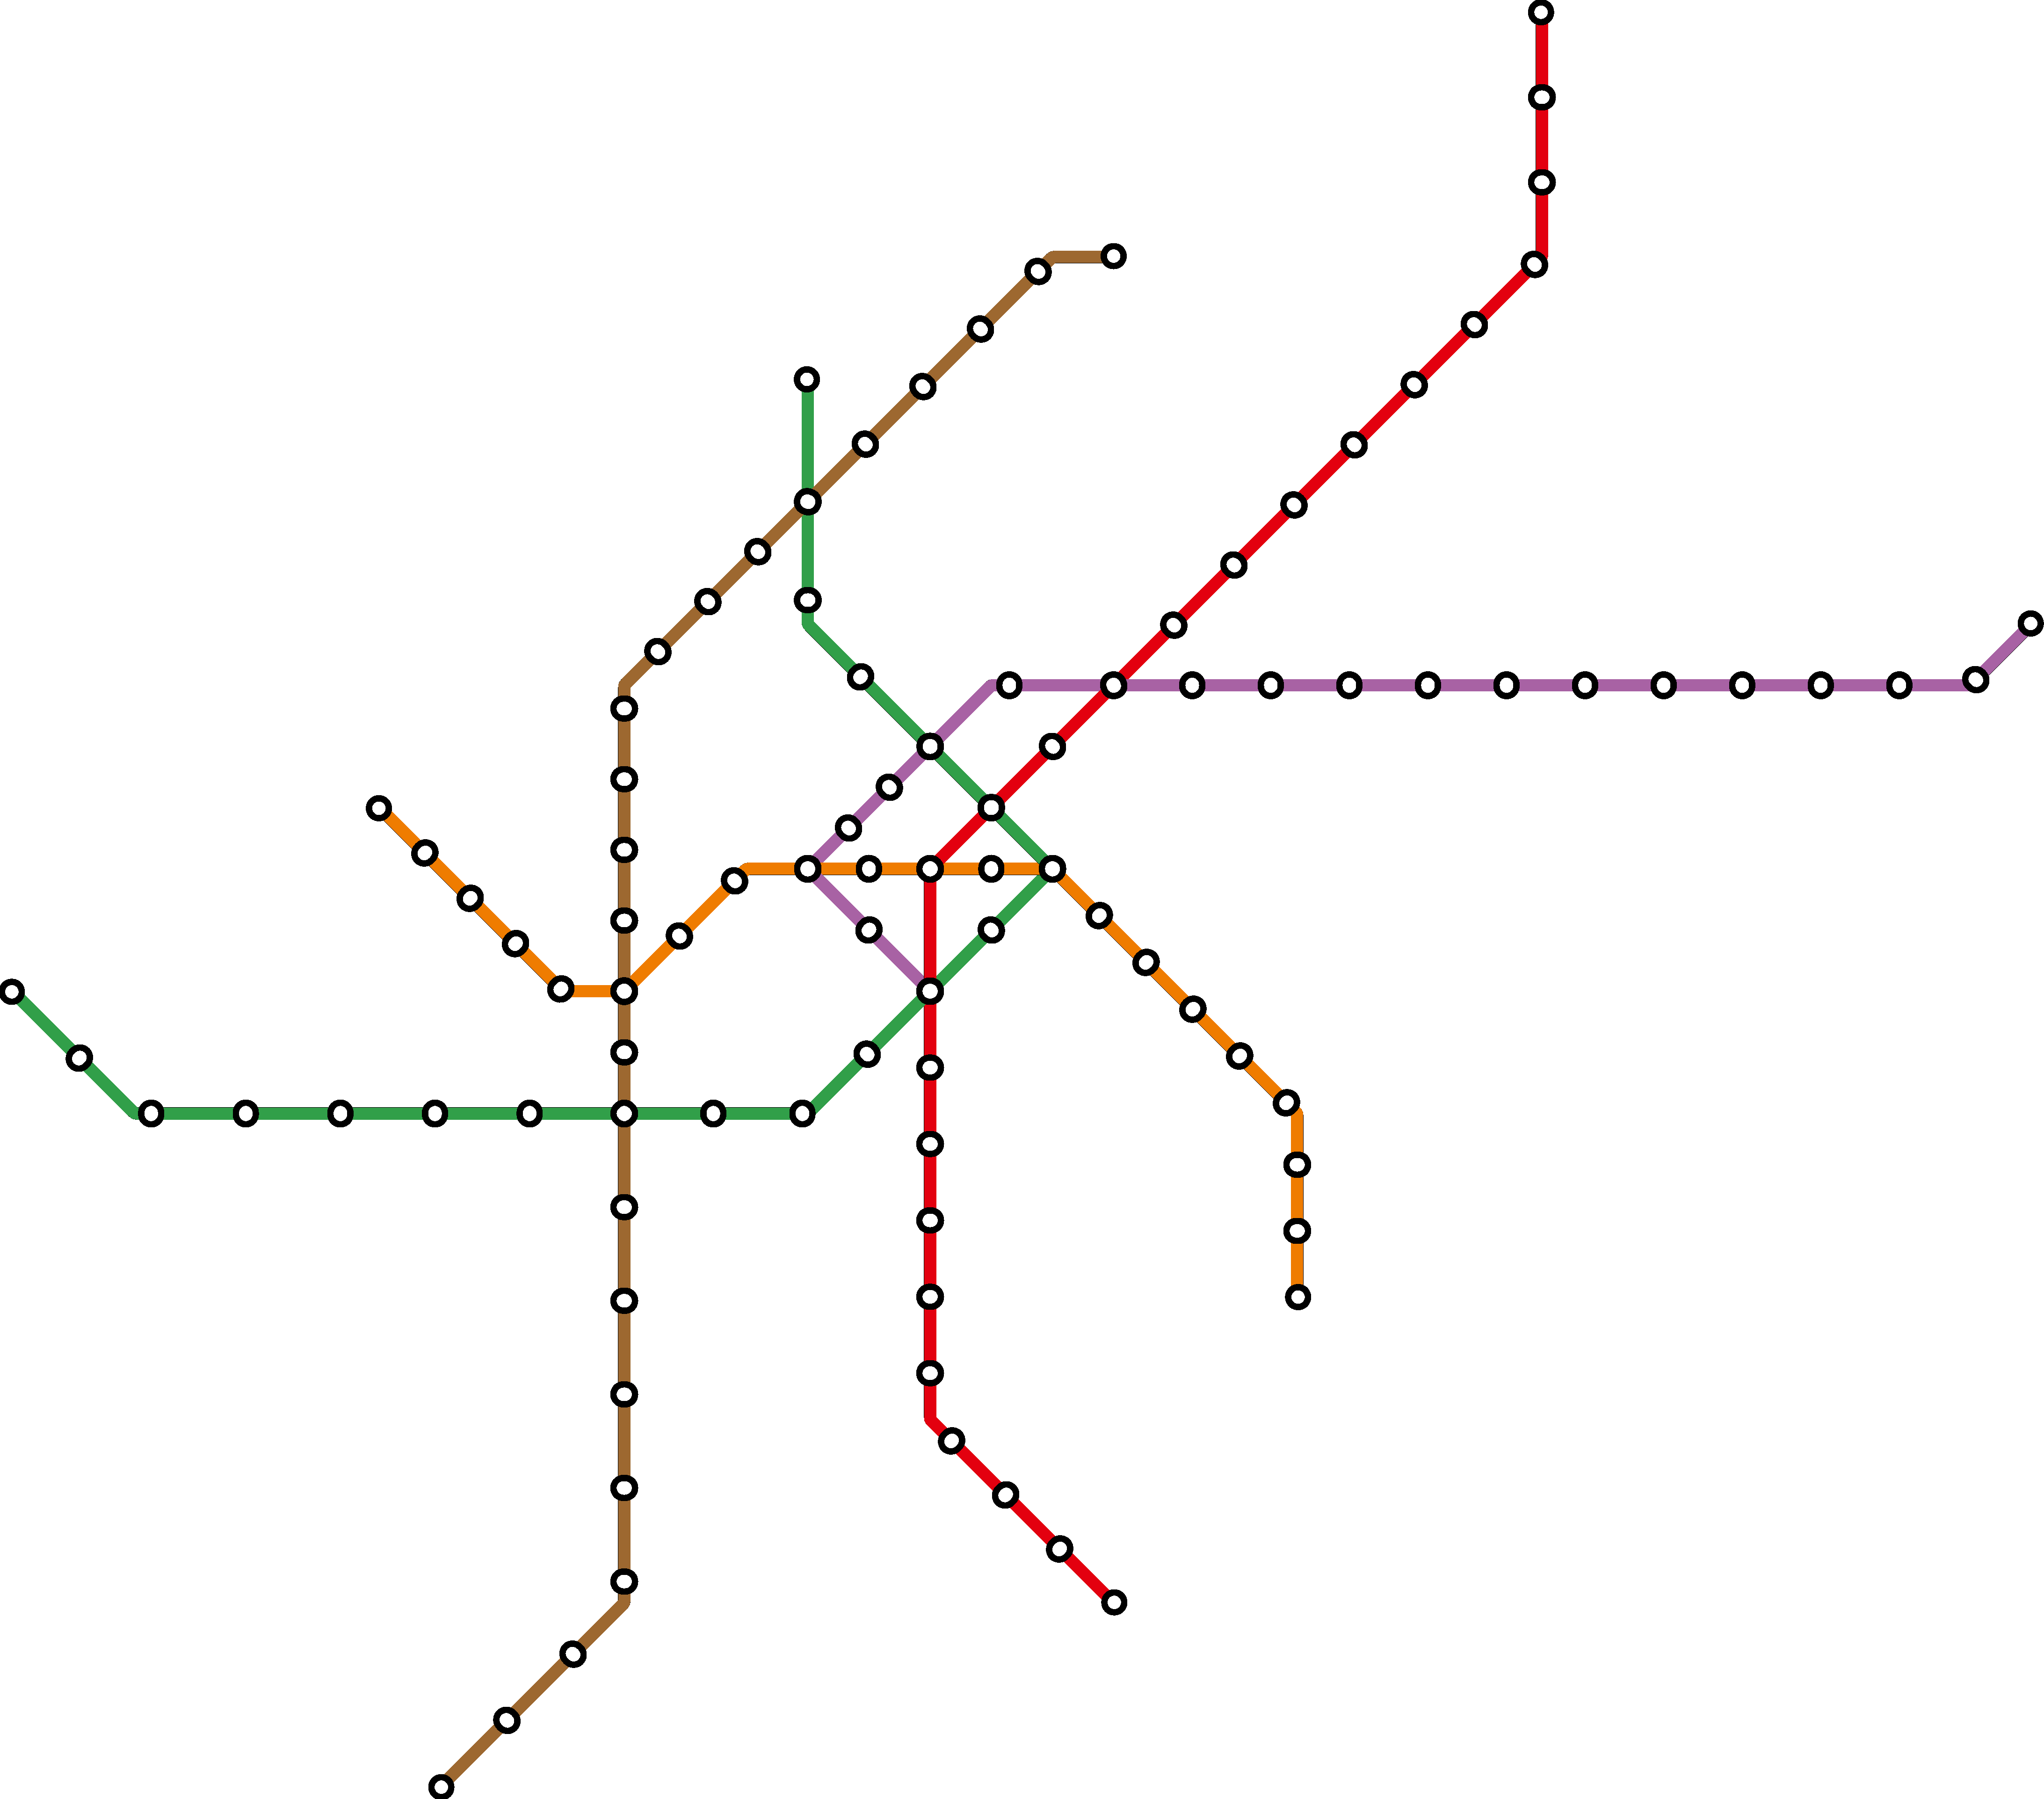
\includegraphics[width=0.27\textwidth]{figures/octi.pdf}
	\vspace{-.5cm}
	\caption{Left: The Vienna subway network, drawn with real-world geographical station positions and line courses. Right: Octilinear drawing by our approx. approach. Octilinearization took 202 ms.}
	\label{FIG:wien}
	\vspace{-.65cm}
\end{figure}

\subsection{Contributions}
\label{SEC:contrib}
%
We consider the following as our main contributions:
\begin{itemize}[parsep=0.5mm,leftmargin=0mm,itemindent=4mm]
\item A
\item B
\end{itemize}

\subsection{Problem definition}
\label{SEC:def}

\subsection{Related Work}
\label{SEC:related}

As metro map layouts and octilinear drawings are of high practical relevance, they both have been studied extensively in the past. 

For metro maps, it was observed early that multiple criteria are important to produce visually pleasing and informative layouts. In \cite{stott2004metro}, a fitness score was introduced which incorporates the number of edge crossings, edge lengths, node distribution, angular resolution, direction changes, and other layout aspects to judge its quality. A hill climbing heuristic was applied to find a layout with a high fitness score. Similar heuristic approaches were described in \cite{hong2004metro}, \cite{hong2006automatic} and  \cite{stott2010automatic}. While such approaches might result in useful layouts, they come without any quality guarantees; and expressing all layout aspects with a single fitness score might obfuscate better trade-offs. In \cite{nollenburg2005mixed} and \cite{noll11}, the metro map layout aspects were subdivided in hard and soft constraints, and a mixed-integer program was used to ensure that all hard constraints (among them octilinearity of all edges) are fulfilled. This method comes with some restrictions on the input graph (planarity, maximum degree of 8, the latter being also a restriction of our approach) and only allows edges without bends. The observed running times were high already for small networks. In \cite{benkert2006minimizing, bekos2007line}, the metro-line crossing minimization problem (MCLM) was introduced. Here, the  goal is to draw a set of simple paths (representing metro lines) along the edges of an embedded underlying graph with a minimum number of pairwise crossings. In \cite{bast2019efficient}, a pipeline was presented in which a problem similar to MCLM was solved efficiently to obtain transit maps with few line crossings and few line separations. However, the goal there was to come up with transit maps in which the abstraction from the real-world course of the lines was negligible. Hence map schematization and in particular octilinearity were not considered in this context.

Octilinear drawings, in which every edge of a given graph is drawn as an alternating sequence of horizontal, vertical and diagonal line segments, have been studied in different contexts before. In \cite{bekos2014planar}, it was proven that for planar input graphs with low degree there always exists an octilinear drawing with at most one direction change (or bend) per edge when using an integer grid where the number of grid nodes is polynomial in the number of input points. The general problem of finding planar octilinear drawings with a minimum number of bends is NP-hard. In \cite{nollenburg2005automated}, an NP-hardness proof for the problem of deciding whether a given embedded graph can be drawn using only straight octilinear edges was given. Our goal is to find an optimal octilinear drawing, i.e., edges are allowed to be represented by octilinear paths rather than just by a single segment but planarity is not a necessary prerequisite. In this configuration, our problem has resemblance to the $k$-node disjoint path problem. There, given a graph and $k$ node pairs, the goal is to find a set of  node-disjoint paths connecting each pair. The problem was proven to be NP-hard even on grid graphs \cite{chuzhoy2015approximating}. As our model allows to assign arbitrary costs to the edges in the octilinear grid graph, the $k$-node disjoint path problem on grids can be seen as a special case of our problem with diagonal costs set to infinity. Our problem therefore is NP-hard, too.

A recent vision paper on passenger navigation in metro networks \cite{craig2019vision} emphasizes the importance of (dynamically adaptable) octilinear drawings of metro maps for guiding passenger flows. But current methods which are fast enough to produce schematic metro maps on demand (as e.g. described in \cite{claudio2014octilinear}, \cite{van2018realtime}, \cite{wang2011} and \cite{wang2016}) either compromise octilinearity or topology preservation, and do not allow for adapting the visualization to different application scenarios. Our pipeline will be shown to be very flexible, and to  produce nearly optimal octilinear drawings quickly.

The metro map layout problem is often considered in conjunction with station labeling. In \cite{noll11}, an extension of the mixed-integer linear program for drawing the metro lines allows to guarantee enough space around station markers for labels. In \cite{WuTLY12} and \cite{WuTHALY13}, this was extended to work with large annotation labels like photographs. In \cite{wang2011} and \cite{wang2016}, labels are placed after the metro map layout was obtained by minimizing an energy function which captures labeling aspect as their directions, spaces between labels and coherence among labels of the same line. While labeling is not the main focus of this paper, we sketch how labels can be included in our model towards the end of the paper.

Finally it should be noted that metro map layout algorithms are not only relevant for visualizing the tracks of real trains, but also for visualizing 'trains of thought'. In fact, the term \emph{metro map metaphor} was coined specifically to capture non-spatial information visualization problems with similar visualization demands as metro maps \cite{sandvad2001metro,nesbitt2004getting,stott2005automatic}. While our evaluation in this paper sticks to actual metro maps, our pipeline works for any graph with given node coordinates and optional edge shapes.
%

\bibliographystyle{ACM-Reference-Format}
\bibliography{pfaedle}
\end{document}
